%%%%%%%%%%%%%%%%%%%%%%%%%%%%%%%
%This is the article LaTeX template for RSC journals
%Copyright The Royal Society of Chemistry 2010
%%%%%%%%%%%%%%%%%%%%%%%%%%%%%%%


\documentclass[8.5pt,twoside,twocolumn]{article}
\oddsidemargin -1.2cm
\evensidemargin -1.2cm
\textwidth 18cm
\headheight 1.0in
\topmargin -3.5cm
\textheight 22cm
\usepackage[super,sort&compress,comma]{natbib} 
\usepackage[version=3]{mhchem}
\usepackage[utf8]{inputenc}
\usepackage{times,mathptmx}
% \usepackage{times}
% feel free not to use mathptmx if it causes difficulties
\usepackage{sectsty}
\usepackage{balance} 

\usepackage{graphicx} %eps figures can be used instead
\usepackage{lastpage}
\usepackage[format=plain,justification=raggedright,singlelinecheck=false,font=small,labelfont=bf,labelsep=space]{caption} 
\usepackage{fancyhdr}
\pagestyle{fancy}

\begin{document}

%\thispagestyle{plain}
%\fancypagestyle{plain}{
%\fancyhead[L]{
\includegraphics[height=8pt]{headers/LH}}
%\fancyhead[C]{\hspace{-1cm}
\includegraphics[height=20pt]{headers/CH}}
%\fancyhead[R]{
\includegraphics[height=10pt]{headers/RH}\vspace{-0.2cm}}
%\renewcommand{\headrulewidth}{1pt}}
%\renewcommand{\thefootnote}{\fnsymbol{footnote}}
%\renewcommand\footnoterule{\vspace*{1pt}% 
%\hrule width 3.4in height 0.4pt \vspace*{5pt}} 
%\setcounter{secnumdepth}{5}



\makeatletter 
\def\subsubsection{\@startsection{subsubsection}{3}{10pt}{-1.25ex plus -1ex minus -.1ex}{0ex plus 0ex}{\normalsize\bf}} 
\def\paragraph{\@startsection{paragraph}{4}{10pt}{-1.25ex plus -1ex minus -.1ex}{0ex plus 0ex}{\normalsize\textit}} 
\renewcommand\@biblabel[1]{#1}            
\renewcommand\@makefntext[1]% 
{\noindent\makebox[0pt][r]{\@thefnmark\,}#1}
\makeatother 
\renewcommand{\figurename}{\small{Fig.}~}
\sectionfont{\large}
\subsectionfont{\normalsize} 

%\fancyfoot{}
%\fancyfoot[LO,RE]{\vspace{-7pt}
\includegraphics[height=9pt]{headers/LF}}
%\fancyfoot[CO]{\vspace{-7.2pt}\hspace{12.2cm}
\includegraphics{headers/RF}}
%\fancyfoot[CE]{\vspace{-7.5pt}\hspace{-13.5cm}
\includegraphics{headers/RF}}
%\fancyfoot[RO]{\footnotesize{\sffamily{1--\pageref{LastPage} ~\textbar  \hspace{2pt}\thepage}}}
%\fancyfoot[LE]{\footnotesize{\sffamily{\thepage~\textbar\hspace{3.45cm} 1--\pageref{LastPage}}}}
\fancyhead{}
\renewcommand{\headrulewidth}{1pt} 
\renewcommand{\footrulewidth}{1pt}
\setlength{\arrayrulewidth}{1pt}
\setlength{\columnsep}{6.5mm}
\setlength\bibsep{1pt}

\twocolumn[
  \begin{@twocolumnfalse}
\noindent\LARGE{\textbf{Self-sustained carbon monoxide oxidation oscillations on size-selected platinum nanoparticles at atmospheric pressure\\ - Supplemental Material}}
\vspace{0.6cm}
 \end{@twocolumnfalse}
  ]


\section{The $\mu$-reactor platform}
The experiments were performed in Si-based 20x15 mm $\mu$-reactors\cite{Henriksen2009}. The reactor consists of two inlets, a mixing zone allowing for diffusional mixing of reactants, an outlet, a reactor volume of $240\,$nL and a $5.4\,\mu$m wide capillary used for sniffing gases from the reactor volume. The reactor is sealed by anodic bonding of a pyrex lid to the Si reactor and is able to operate at a pressure range of 0-2.5\,bar. The reaction gases is supplied to the two inlets by flow controllers capable of controlling the gas flow from 0-10 mL/min. The capillary flow is fed into a quadropole mass-spectrometer (QMA) for analysis while any surplus of gas from the inlets are passed directly through to the outlet via a pressure controller allowing control of reactor pressure. The design makes sure that all gases exposed to the catalyst under investigation is measured by the QMA ensuring an extremely high sensitivity of the system. 

\begin{figure}[h]
  \centering
  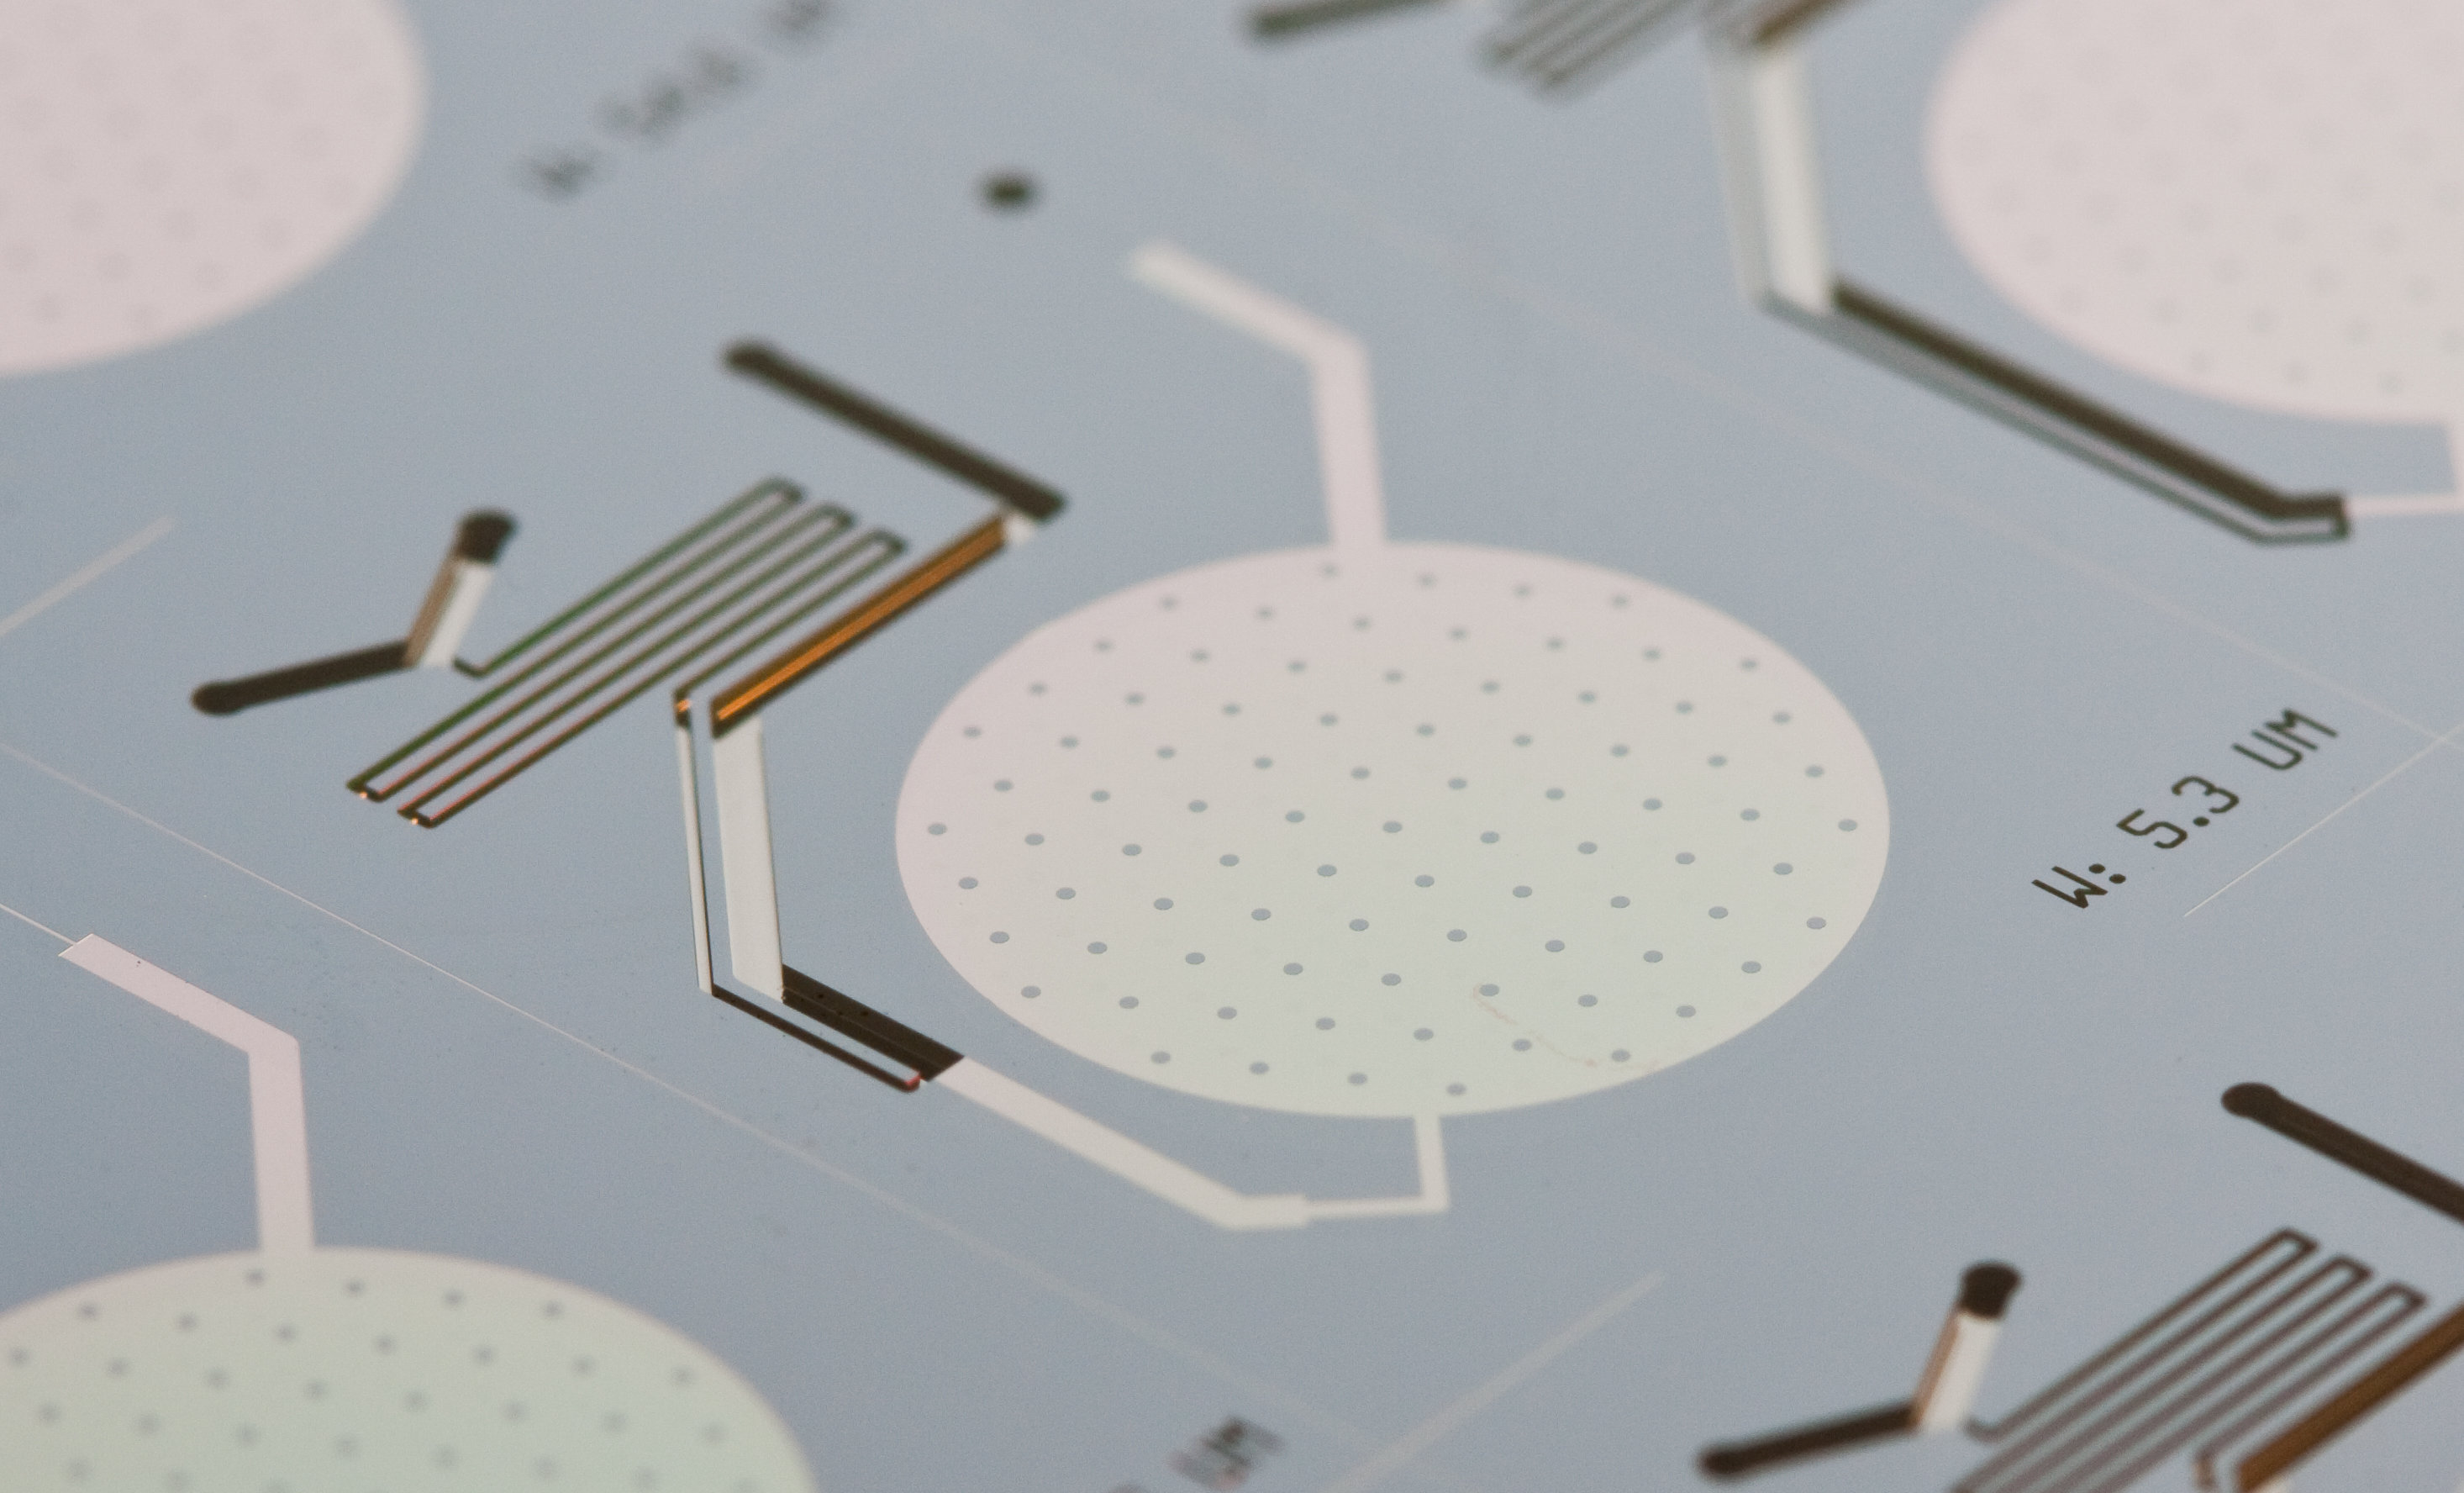
\includegraphics[width=9cm]{reactor.jpg}
  \caption{The Microreactor before the lid is anodicly bonded to the reactor}
  \label{fgr:reactor}
\end{figure}


Before any measurements are performed the reactor is pumped by a turbopump to minimize contaminants in the system. When an evacuated reactor is mounted the base pressure of the mass spectrometer chamber is $\sim5\times10^{-9}\,$mbar and in operation at $1\,$bar in the reactor volume the pressure is $\sim5\times10^{-7}\,$mbar in the QMA chamber. 

The reactor is heated by joule heating of a Pt strip evaporated on the backside of the reactor volume. The introduction of two additional contacts on the backside of the reactor allows for 4 wire measurements of the resistance of the Pt strip using it as a RTD for temperature measurement of the reactor. An external thermocouple acts as room-temperature calibration of the RTD as well as sanity check of the RTD measurement during operation.

The gas handling including flow and pressured controllers and the mass spectrometer is fully automized allowing for measurements of several days without human intervention allowing for self-consistent measurements of many samples.

\section{Pt nanoparticle deposition}
Pt nanoparticles were deposited in the reactor using a gas-aggregation source (Mantis Deposition Ltd., Nanogen 50). Pt clusters were formed by gas-phase condensation of Pt atoms produced by impinging argon ions on a 99.99\% Pt target in a magnetron sputter source. After condensation the ionised fraction (60-80\%) of the clusters were size-selected by a quadropole mass selection filter according to their mass-to-charge ratio. Using this setup Pt nanoparticles with diameters in the range of 2--16\,nm can be produced \cite{Nielsen2010,Nielsen2009}. The size-selected nanoparticles were after size-selection soft-landed in the reactor volume of the microreactor. The coverage was kept at approximately 0.1\% geometric coverage determined by measuring the current on the reactor during deposition. After deposition the reactors were anodicly cold-bonded \cite{Vesborg2010} to a pyrex lid to avoid sintering of the nanoparticles while bonding.

\section{CO concentration dependence}
The dependence of the CO concentration on the period of the oscillations was investigated. The result show that the period increases slightly with increasing CO-concentration. However, the effect is small compared to the general trend of slower oscillations as the experiment progresses. In Figure~\ref{fgr:gas_dependence_summary} the oscillation periods are summarized and the actual masspectrometry data of the entire experiment is shown in Figure~\ref{fgr:gas_dependence}.

\begin{figure}[h]
  \centering
  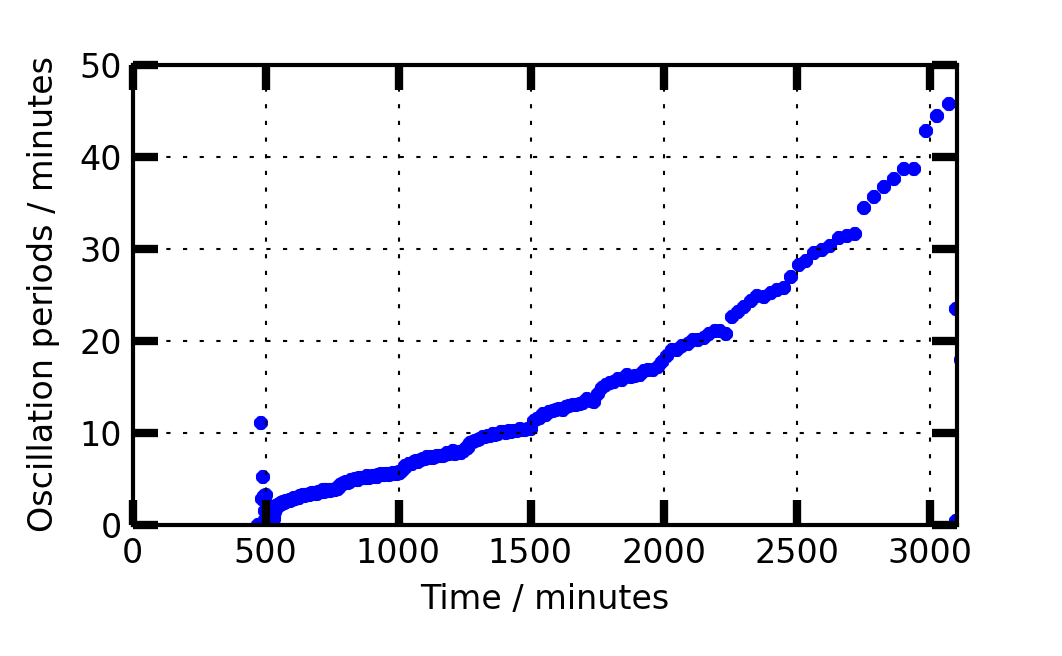
\includegraphics[width=9cm]{oscillations_gas_dependence_summary_supplemental.png}
  \caption{Summary of the gas-dependence. The overall trend of increasing oscillation period is now supporimposed by small discontinous stpes when the CO concentration is increased.}
  \label{fgr:gas_dependence_summary}
\end{figure}

\begin{figure*}
  \centering
  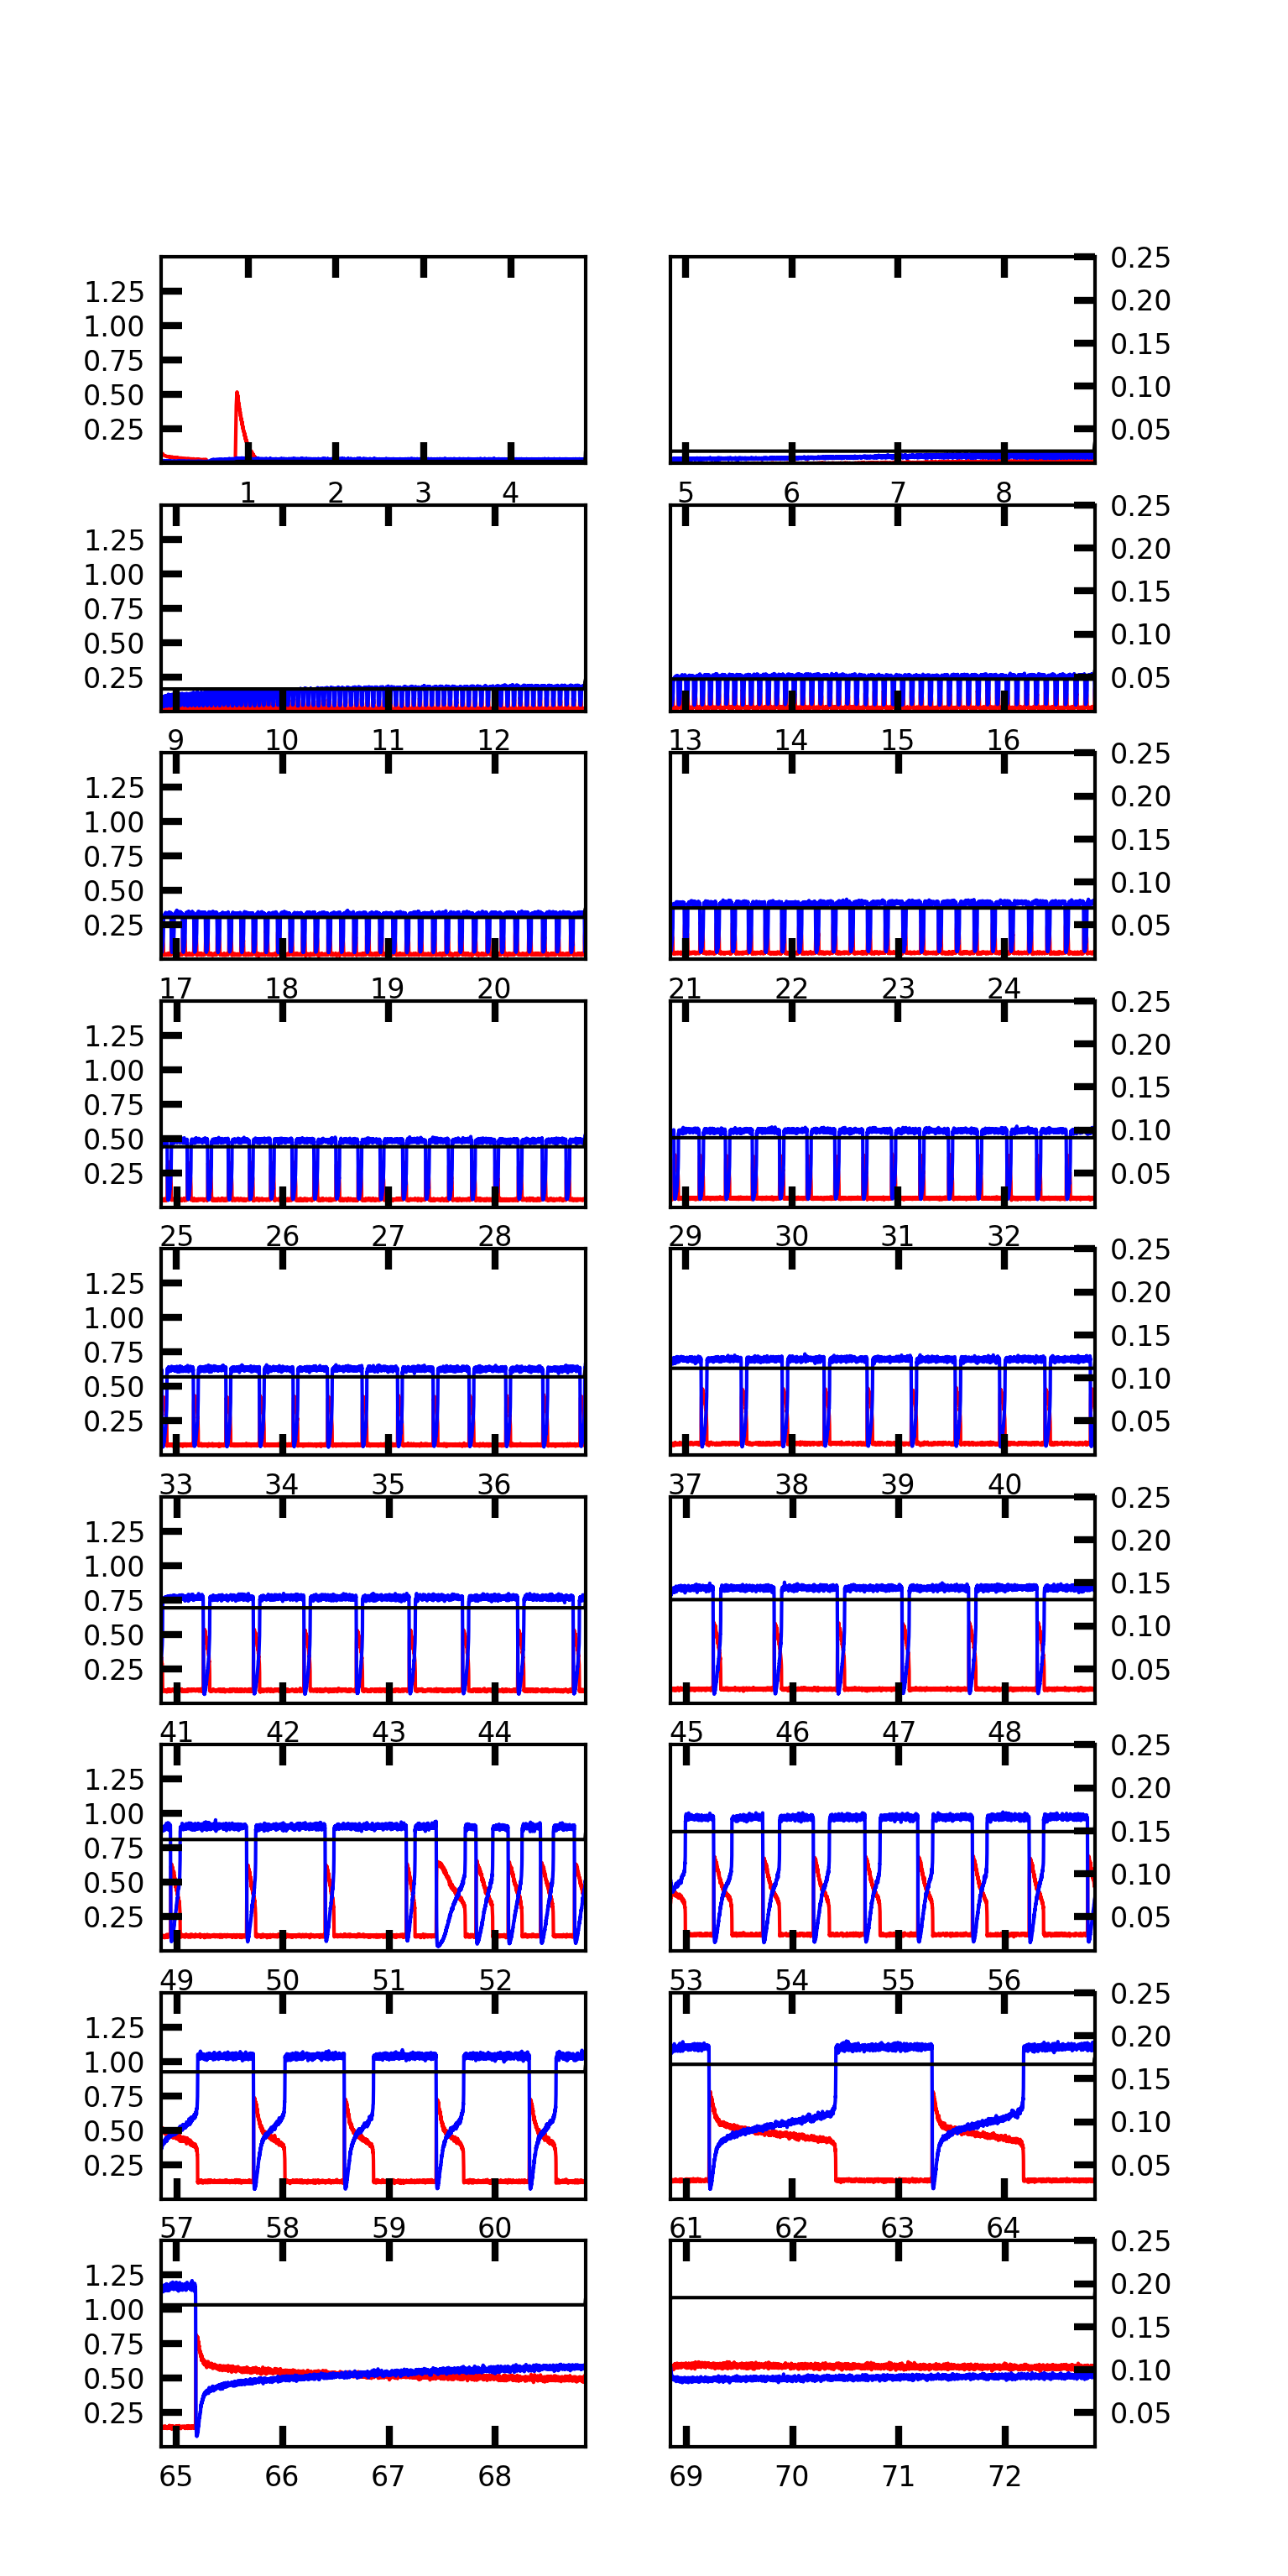
\includegraphics[width=14cm]{oscillations_gas_dependence_supplemental.png}
  \caption{Complete series of oscillating sample, showing CO (red) and CO$_2$ (blue). The temperature is constant $210^\circ$C doing the entire measurement. For every frame the CO-concentration is increased.}
  \label{fgr:gas_dependence}
\end{figure*}

\section{Temperature dependence}
As mentioned in the main paper, the oscillations shows a very strong temperature dependence. In Figure~\ref{fgr:temperature_dependence_supplemental} we show an example where the oscillations are turned on and off by changing the temperature $20^\circ$C.

\begin{figure}[h]
\centering
  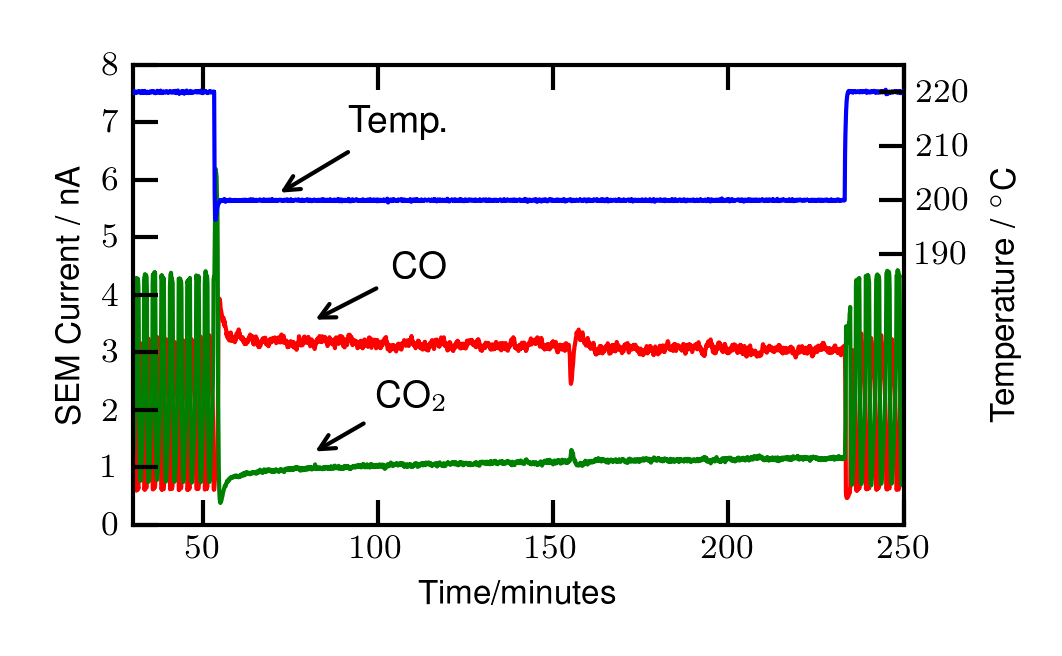
\includegraphics[width=9cm]{temperature_dependence_supplemental.png}
  \caption{Another example of the very pronounced temperature dependence.}
  \label{fgr:temperature_dependence_supplemental}
\end{figure}

\section{Duty cycle}
Even though the period of the oscillations increases with time, the total integrated conversion doing a complete cycle is almost constant. In Figure~\ref{fgr:duty_cycles_supplemental}, the value of the integral of CO and CO$_2$ is plotted for every oscillation in the four-day long experiment. It is evident that the ratio between CO and CO$_2$ is almost constant and thus the overall activity of the sample is almost unchanged despite the development in the oscillation frequency.


\begin{figure}[h]
\centering
  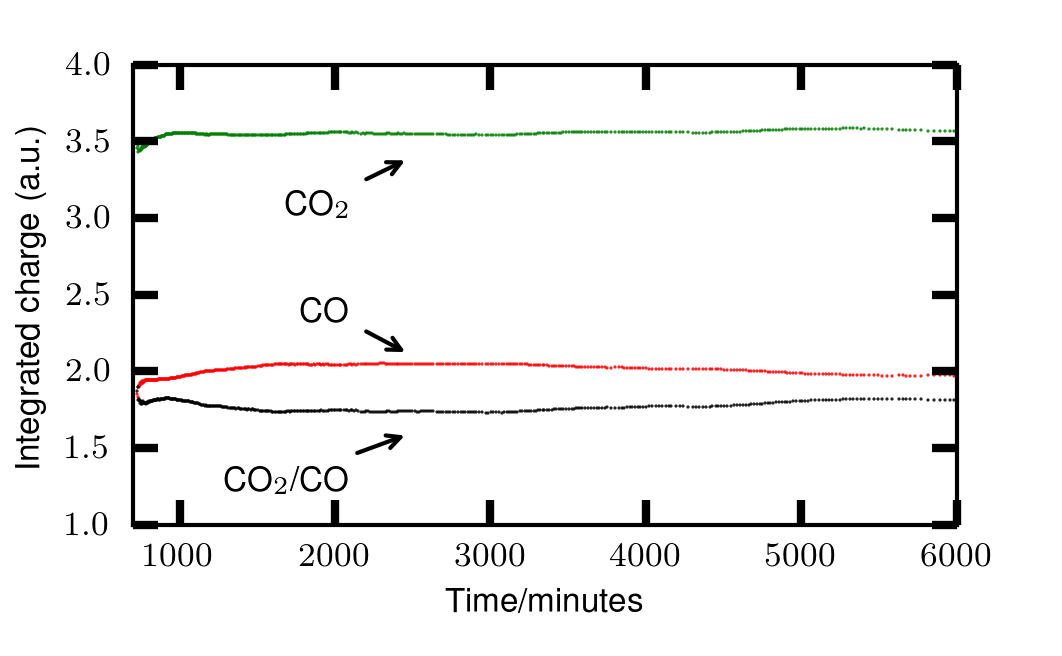
\includegraphics[width=9cm]{duty_cycles_long_measurement_supplemental.png}
  \caption{A plot of the duty-cycle of the sample duing the 4-day long experiment. The individual data-points is calculted as the integral of CO (red) or CO$_2$ (blue) doing the individual oscillations. The ratio between CO and CO$_2$ is drawn in black.}
  \label{fgr:duty_cycles_supplemental}
\end{figure}



\footnotesize{
\bibliography{literature} %your .bib file
\bibliographystyle{rsc} %the RSC's .bst file
}

\end{document}
